% libroResMat2
% Copyright (C) 2020  J.M. Perez Zerpa, et. al.
%
% This program is free software: you can redistribute it and/or modify
% it under the terms of the GNU General Public License as published by
% the Free Software Foundation version 3 of the License.
%
% This program is distributed in the hope that it will be useful,
% but WITHOUT ANY WARRANTY; without even the implied warranty of
% MERCHANTABILITY or FITNESS FOR A PARTICULAR PURPOSE. See the
% GNU General Public License for more details.
%
% You should have received a copy of the GNU General Public License
% along with this program.  If not, see <http://www.gnu.org/licenses/>.

\chapter{Inestabilidad}

\textbf{JORGE: puse un ejemplo que había redactado para 2017, con el enfoque anterior... Bruno: tomalo o dejalo sin compromiso!}


El contenido del presente capítulo complementa los contenidos incluidos en el documento publicado para la Unidad Temática 7 en el curso 2017.
 
\section{Ejemplo: ménsula con carga axial}

Se considera una ménsula formada por un material de módulo de Young $E$, de largo $\ell$ con sección transversal de inercia $I$ sometida a una carga axial de compresión $N$ aplicada en su extremo libre con una excentricidad $e$, como se muestra en la Figura~\ref{fig:esqpand}. %
%
No hay carga transversal aplicada, por lo tanto $q=0$. %

\begin{figure}[htb]
\centering
\def\svgwidth{0.5\textwidth}
\input{figs/UT7/ejemplo_pandeo.pdf_tex}
\caption{Esquema de ménsula con carga axial con excentricidad.}
\label{fig:esqpand}
\end{figure}

En estructuras reales, excentricidades como la considerada pueden ser provocadas por errores en la ejecución de elementos estructurales conectados a la ménsula (por ejemplo vigas descargando sobre columnas). %
%
Esto permite considerar la excentricidad como una \textit{imperfección}, la cual usualmente tiene magnitud considerablemente menor a las dimensiones de la sección transversal. %
% ------------------------------------------


La ecuación diferencial de la deflexión $v$ dada por el equilibrio está dada por:
%
\begin{equation}
  E I \frac{\partial^4 v}{\partial x^4}(x)
+   N \frac{\partial^2 v}{\partial x^2}(x)
=   0.
\end{equation}
%
La solución y sus derivadas están dadas por:
%
\begin{eqnarray}
                               v  (x) &=& A \cos(k x ) + B \sin(kx) + C x + D, \\
\frac{\partial   v}{\partial x  } (x) &=& -A k \sin(k x ) + B k \cos(kx) + C , \\
\frac{\partial^2 v}{\partial x^2} (x) &=& - A k^2 \cos(k x ) - B k^2 \sin(kx),  \\
\frac{\partial^3 v}{\partial x^3} (x) &=& A k^3 \sin(k x ) - B k^3 \cos(kx), 
\end{eqnarray}
donde
$$
  k^2 = \frac{N}{EI}.
$$

Además se cumplen las relaciones:
$$
M(x)=\frac{\partial^2 v}{\partial x^2}(x) EI \quad \text{y} \quad V(x) = EI \frac{\partial^3 v}{\partial x^3}(x) + N \frac{\partial v}{\partial x}(x).
$$

Condiciones de contorno en función de flechas o solicitaciones:
%
\begin{equation}
\left\{
\begin{array}{l}
v(0)=0 \\[.5em]
\displaystyle \frac{\partial v}{\partial x}(0)=0\\[1em]
V(\ell)=0\\[.5em]
M(\ell)=-N e.
\end{array}
\right.
\end{equation}

Es necesario obtener las condiciones de contorno en función de la flecha. %
Se comienza desarrollando la condición del cortante, es decir
%
\begin{equation}
	V(\ell) = 0,
\end{equation}
donde operando se obtiene la relación equivalente, en función de la flecha:
%
\begin{equation}
  \frac{\partial^3 v}{\partial x^3} (\ell) = - k^2 \frac{\partial v}{\partial x}(\ell).
\end{equation}
%
Sustituyendo la expresión de la solución se tiene:
%	
\begin{equation}
	Ak^3 \sin(k\ell) - Bk^3 \cos(k\ell) = Ak^3 \sin(k\ell) - Bk^3 \cos(k\ell) - C k^2,
\end{equation}
por lo tanto se cumple:
\begin{equation}\label{eqn:ejemplopand}
\boxed{
  C=0
}
\end{equation}

Usando la condición de giro nulo en el empotramiento se tiene
\begin{equation}
v'(0)=0 \Leftrightarrow  Bk + C = 0,
\end{equation}
%
por lo tanto usando la Ecuación~\eqref{eqn:ejemplopand} se tiene
\begin{equation}
\boxed{
B=0
}
\end{equation}

Usando la condición de momento en $\ell$ se tiene
%
\begin{equation}
M(\ell) = -N e \Leftrightarrow \frac{\partial v^2}{\partial x^2} (\ell)  = - k^2 e
\end{equation}
%
por lo tanto
%
\begin{equation}
-k^2 A \cos(k\ell) - k^2 B \cos(k\ell) = -k^2 e
\end{equation}

Esto es equivalente a 
\begin{equation}\label{eqn:acos}
\boxed{
A \cos(k\ell)  = e
}
\end{equation}

Finalmente usando la condición de desplazamiento nulo en el empotramiento se tiene
%
\begin{equation}
v(0)=0  \Leftrightarrow \boxed{ A + D = 0}
\end{equation}

Es necesario estudiar de forma independiente las soluciones obtenidas para los casos con y sin imperfecciones.

\subsection{Solución sin imperfección}

El caso sin imperfección corresponde a $e=0$ y la expresión solución está dada por:
%
\begin{equation}
v(x) = A (\cos(k x) -1), \quad \text{con} \quad A\cos(k\ell) = 0.
\end{equation}

Si se verifica
%
\begin{equation}
k \ell = \frac{\pi}{2} + n\pi  \quad \text{con} \,\, n\in \bbN,
\end{equation}
%
entonces cualquier valor de $A$ cumple la condición por lo que existen infinitas soluciones. %
%
En particular la menor directa asociada estos valores de $k$ es
\begin{equation}
\boxed{
N_{cr} = \frac{\pi^2 E I}{4 \ell^2}.
}
\end{equation}
%
Esta carga crítica corresponde a una luz de pandeo $L_p = 2\ell$.



\subsection{Solución con imperfección}

En este caso se considera una excentricidad $e \neq 0$, por lo que se obtiene una única solución dada por:
%
\begin{equation}
v(x) = \frac{e}{\cos(k\ell)} (\cos(k x) -1).
\end{equation}
%
Se destaca que se asumió que $\cos(k \ell) \neq 0$, en caso contrario se tendría una incompatibilidad en la Ecuación~\eqref{eqn:acos}. %

Se mostrará que, de acuerdo con el modelo considerado (de grandes desplazamientos y pequeños giros), existe un nivel de carga para el cual la estructura pierde capacidad de soportar cargas superiores (rigidez) y la flecha adquiere valores elevados. %
%

Como referencia se considera la flecha en el extremo libre, es decir:
%
\begin{equation}
v(\ell) = e \left( 1- \frac{1}{\cos(k\ell) }  \right)
\end{equation}
%
si $k=0$ se tiene un valor nulo de flecha, mientras que al aumentar el valor de $N$ se tiene un crecimiento que lleva a que cuando se alcanza el valor 
%
\begin{equation}
k = \frac{\pi}{2 \ell }
\end{equation}
%
la flecha tiende a infinito. %
%
Esto establece por lo tanto que la carga crítica de la estructura es la misma del caso anterior
%
\begin{equation}
\boxed{
	N_{cr} = \frac{\pi^2 E I}{4 \ell^2}.
}
\end{equation}


En la Figura~\ref{fig:ejpand} se presenta la curva de desplazamientos del extremo libre (abscisas) para diferentes valores de $k\ell$ (ordenadas). %
%
Para $k\ell$ se consideran 30 valores equiespaciados entre $0$ y $\frac{\pi}{2} 0.99$.

\begin{figure}[htb]
	\centering
		\resizebox{.7\textwidth}{!}{% Title: gl2ps_renderer figure
% Creator: GL2PS 1.3.9, (C) 1999-2015 C. Geuzaine
% For: Octave
% CreationDate: Mon Dec  4 08:08:25 2017
\setlength{\unitlength}{1pt}
\begin{picture}(0,0)
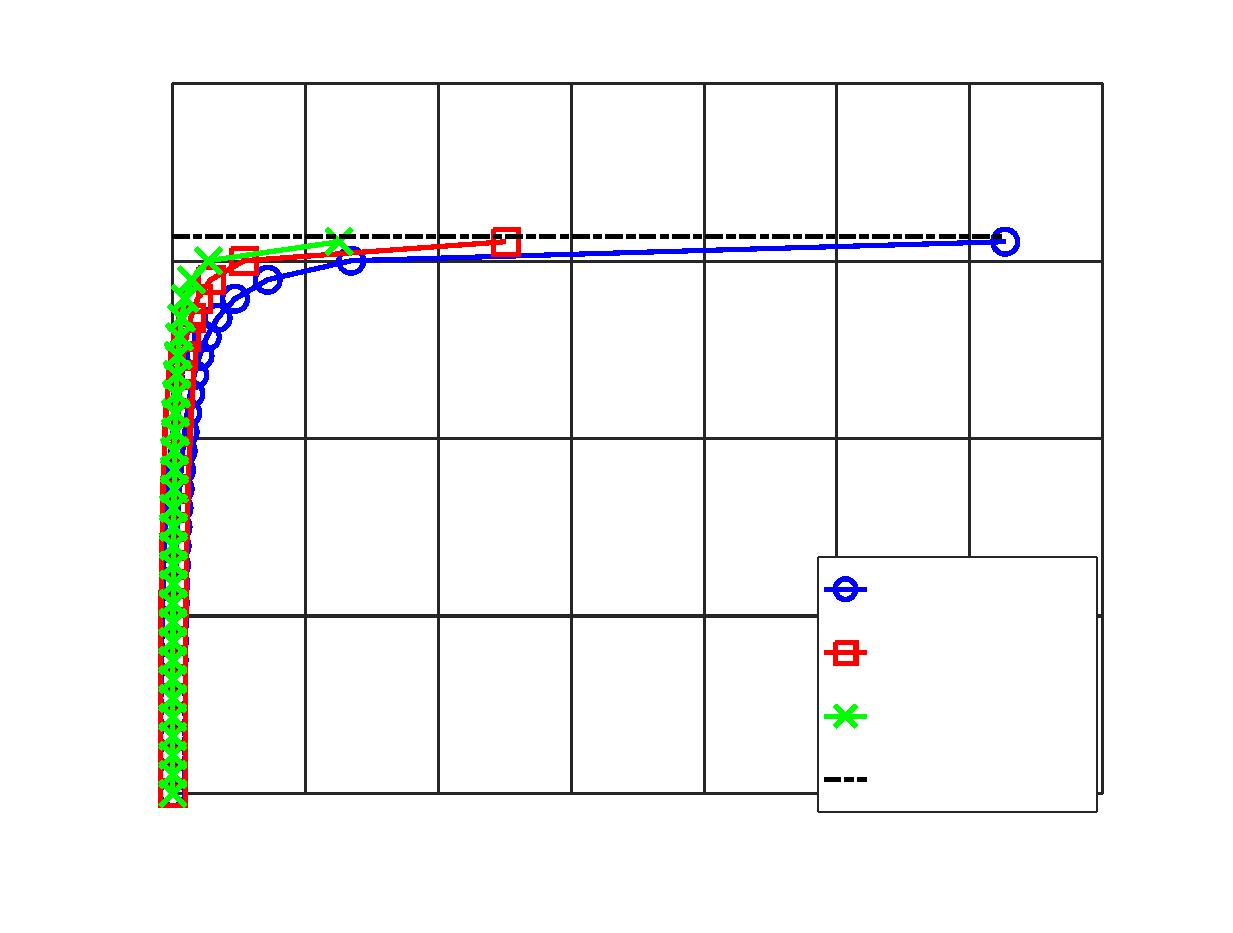
\includegraphics{plotejempand-inc}
\end{picture}%
\begin{picture}(576,432)(0,0)
\fontsize{22}{0}
\selectfont\put(74.88,54.0046){\makebox(0,0)[t]{\textcolor[rgb]{0.15,0.15,0.15}{{0}}}}
\fontsize{22}{0}
\selectfont\put(138.651,54.0046){\makebox(0,0)[t]{\textcolor[rgb]{0.15,0.15,0.15}{{5}}}}
\fontsize{22}{0}
\selectfont\put(202.423,54.0046){\makebox(0,0)[t]{\textcolor[rgb]{0.15,0.15,0.15}{{10}}}}
\fontsize{22}{0}
\selectfont\put(266.194,54.0046){\makebox(0,0)[t]{\textcolor[rgb]{0.15,0.15,0.15}{{15}}}}
\fontsize{22}{0}
\selectfont\put(329.966,54.0046){\makebox(0,0)[t]{\textcolor[rgb]{0.15,0.15,0.15}{{20}}}}
\fontsize{22}{0}
\selectfont\put(393.737,54.0046){\makebox(0,0)[t]{\textcolor[rgb]{0.15,0.15,0.15}{{25}}}}
\fontsize{22}{0}
\selectfont\put(457.509,54.0046){\makebox(0,0)[t]{\textcolor[rgb]{0.15,0.15,0.15}{{30}}}}
\fontsize{22}{0}
\selectfont\put(521.28,54.0046){\makebox(0,0)[t]{\textcolor[rgb]{0.15,0.15,0.15}{{35}}}}
\fontsize{22}{0}
\selectfont\put(69.8755,58.9987){\makebox(0,0)[r]{\textcolor[rgb]{0.15,0.15,0.15}{{0}}}}
\fontsize{22}{0}
\selectfont\put(69.8755,144.149){\makebox(0,0)[r]{\textcolor[rgb]{0.15,0.15,0.15}{{0.5}}}}
\fontsize{22}{0}
\selectfont\put(69.8755,229.299){\makebox(0,0)[r]{\textcolor[rgb]{0.15,0.15,0.15}{{1}}}}
\fontsize{22}{0}
\selectfont\put(69.8755,314.45){\makebox(0,0)[r]{\textcolor[rgb]{0.15,0.15,0.15}{{1.5}}}}
\fontsize{22}{0}
\selectfont\put(69.8755,399.6){\makebox(0,0)[r]{\textcolor[rgb]{0.15,0.15,0.15}{{2}}}}
\fontsize{22}{0}
\selectfont\put(298.08,27.0046){\makebox(0,0)[t]{\textcolor[rgb]{0.15,0.15,0.15}{{Desplazamiento $v(\ell)$}}}}
\fontsize{22}{0}
\selectfont\put(30.8755,229.299){\rotatebox{90}{\makebox(0,0)[b]{\textcolor[rgb]{0.15,0.15,0.15}{{$k \ell$}}}}}
\fontsize{22}{0}
\selectfont\put(410.88,157.064){\makebox(0,0)[l]{\textcolor[rgb]{0,0,0}{{$e=$ 0.5}}}}
\fontsize{22}{0}
\selectfont\put(410.88,126.549){\makebox(0,0)[l]{\textcolor[rgb]{0,0,0}{{$e=$ 0.2}}}}
\fontsize{22}{0}
\selectfont\put(410.88,96.0347){\makebox(0,0)[l]{\textcolor[rgb]{0,0,0}{{$e=$ 0.1}}}}
\fontsize{22}{0}
\selectfont\put(410.88,65.5203){\makebox(0,0)[l]{\textcolor[rgb]{0,0,0}{{$e=0$}}}}
\end{picture}
}
	\caption{Resultado analítico de inestabilidad con imperfección.}
	\label{fig:ejpand}
\end{figure}

Se puede observar cómo la presencia de imperfecciones de mayor magnitud provocan que la estructura tenga mayores desplazamientos para cada valor de carga dado. %
%
Para todas las excentricidades, la curva tiene una asíntota horizontal en $k\ell=\frac{\pi}{2}$, por lo que este modelo establece que la estructura no es capaz de soportar cargas superiores a la carga crítica.


La curvatura está dada por la función 
\begin{equation}
\frac{\partial^2 v}{\partial x^2}(x) = -k^2 e \frac{\cos(k x)}{\cos(k\ell)}.
\end{equation}


Se puede mostrar que
\begin{equation}
\lim\limits_{N\rightarrow N_{cr}}
\left| \frac{\partial^2 v}{\partial x^2}(x) \right|
 =
\left\{
\begin{array}{lr}
\infty & \text{si } x \in (-\ell,\ell)\\
\displaystyle \frac{\pi^2 e}{4 \ell^2} & \text{si } x \in \{-\ell,\ell\}
\end{array}
\right.
\end{equation}
%
por lo tanto, a partir de este resultado, se puede interpretar que la longitud de pandeo es aquella que separa puntos con curvatura acotada.

\subsection{Modelo numérico considerando grandes giros}

Para verificar el resultado analítico obtenido se realiza un modelo numérico usando la herramienta de análisis no lineal ONSA\footnote{\textit{Open Nonlinear Structural Analyzer}: código de GNU-Octave para el análisis no lineal de reticulados. Disponible en \citep{Bazzano2017}.}.

Se considera un perfil PNI 10 de acero ($E=210 $ GPa), de largo $\ell=5$ m, analizado en flexión respecto a la mayor inercia ($I= 171$ cm$^4$). %
%
Esto corresponde a una carga crítica $N_{cr}=35.4 $ kN. %
%
Se asume que la excentricidad es $e=5$ mm.


Para realizar el análisis usando el ONSA se considera un reticulado con geometría y áreas de barras tales que el comportamiento es equivalente al de la viga a analizar. %
El desarrollo de esta equivalencia es presentado en \citep{Bazzano2017}. %
% -------------------------


En la Figura~\ref{fig:nonlindefejpand} se muestra la curva carga-desplazamiento. %
%
En dicha gráfica se coloca el factor de carga en las ordenadas y el desplazamiento de referencia asociado a la configuración de equilibrio correspondiente en las abscisas. % 
%
El estado de carga de referencia considerado es el dado por la carga crítica de pandeo $N_{cr}$ por lo que un factor de carga unitario corresponde a dicho estado de carga mientras que un factor menor corresponde a una carga menor a la carga crítica. %

\begin{figure}[htb]
	\centering
	\subfloat[Curva Carga-Desplazamiento.]{
		\resizebox{.5\textwidth}{!}{% Title: gl2ps_renderer figure
% Creator: GL2PS 1.3.9, (C) 1999-2015 C. Geuzaine
% For: Octave
% CreationDate: Sun Dec  3 14:27:03 2017
\setlength{\unitlength}{1pt}
\begin{picture}(0,0)
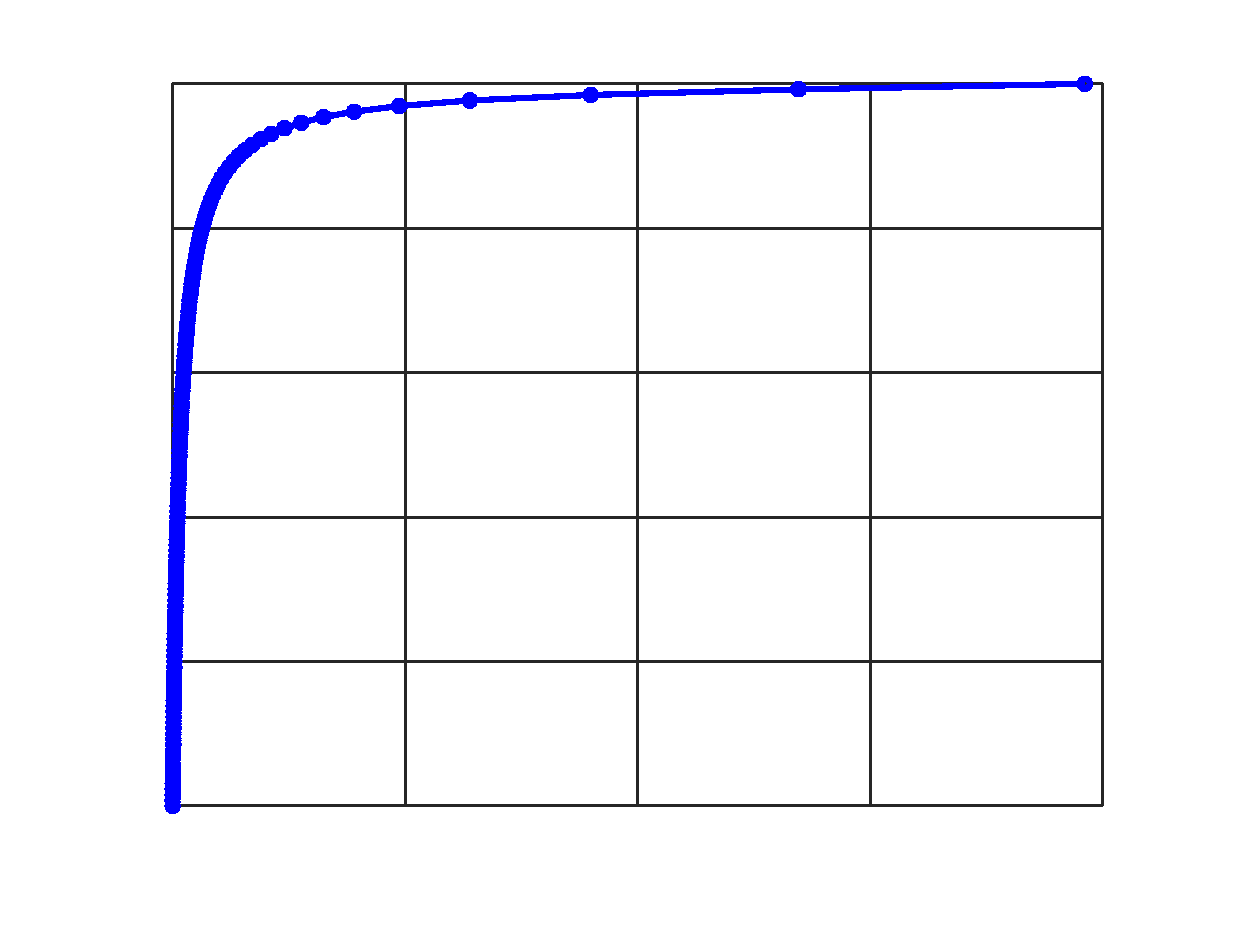
\includegraphics{Cantilever_Buckling_ImperfLoad-inc}
\end{picture}%
\begin{picture}(576,432)(0,0)
\fontsize{20}{0}
\selectfont\put(74.88,48.007){\makebox(0,0)[t]{\textcolor[rgb]{0.15,0.15,0.15}{{0}}}}
\fontsize{20}{0}
\selectfont\put(186.48,48.007){\makebox(0,0)[t]{\textcolor[rgb]{0.15,0.15,0.15}{{0.2}}}}
\fontsize{20}{0}
\selectfont\put(298.08,48.007){\makebox(0,0)[t]{\textcolor[rgb]{0.15,0.15,0.15}{{0.4}}}}
\fontsize{20}{0}
\selectfont\put(409.68,48.007){\makebox(0,0)[t]{\textcolor[rgb]{0.15,0.15,0.15}{{0.6}}}}
\fontsize{20}{0}
\selectfont\put(521.28,48.007){\makebox(0,0)[t]{\textcolor[rgb]{0.15,0.15,0.15}{{0.8}}}}
\fontsize{20}{0}
\selectfont\put(69.8755,53.0012){\makebox(0,0)[r]{\textcolor[rgb]{0.15,0.15,0.15}{{0}}}}
\fontsize{20}{0}
\selectfont\put(69.8755,122.321){\makebox(0,0)[r]{\textcolor[rgb]{0.15,0.15,0.15}{{0.2}}}}
\fontsize{20}{0}
\selectfont\put(69.8755,191.641){\makebox(0,0)[r]{\textcolor[rgb]{0.15,0.15,0.15}{{0.4}}}}
\fontsize{20}{0}
\selectfont\put(69.8755,260.961){\makebox(0,0)[r]{\textcolor[rgb]{0.15,0.15,0.15}{{0.6}}}}
\fontsize{20}{0}
\selectfont\put(69.8755,330.28){\makebox(0,0)[r]{\textcolor[rgb]{0.15,0.15,0.15}{{0.8}}}}
\fontsize{20}{0}
\selectfont\put(69.8755,399.6){\makebox(0,0)[r]{\textcolor[rgb]{0.15,0.15,0.15}{{1}}}}
\fontsize{20}{0}
\selectfont\put(298.08,24.007){\makebox(0,0)[t]{\textcolor[rgb]{0.15,0.15,0.15}{{Displacements}}}}
\fontsize{20}{0}
\selectfont\put(33.8755,226.301){\rotatebox{90}{\makebox(0,0)[b]{\textcolor[rgb]{0.15,0.15,0.15}{{Load factors}}}}}
\end{picture}
}
	\label{fig:nonlindefejpand}
	}
	\subfloat[Geometrías de referencia (azul) y deformada (rojo).]{
    	\resizebox{.5\textwidth}{!}{% Title: gl2ps_renderer figure
% Creator: GL2PS 1.3.9, (C) 1999-2015 C. Geuzaine
% For: Octave
% CreationDate: Sun Dec  3 14:27:00 2017
\setlength{\unitlength}{1pt}
\begin{picture}(0,0)
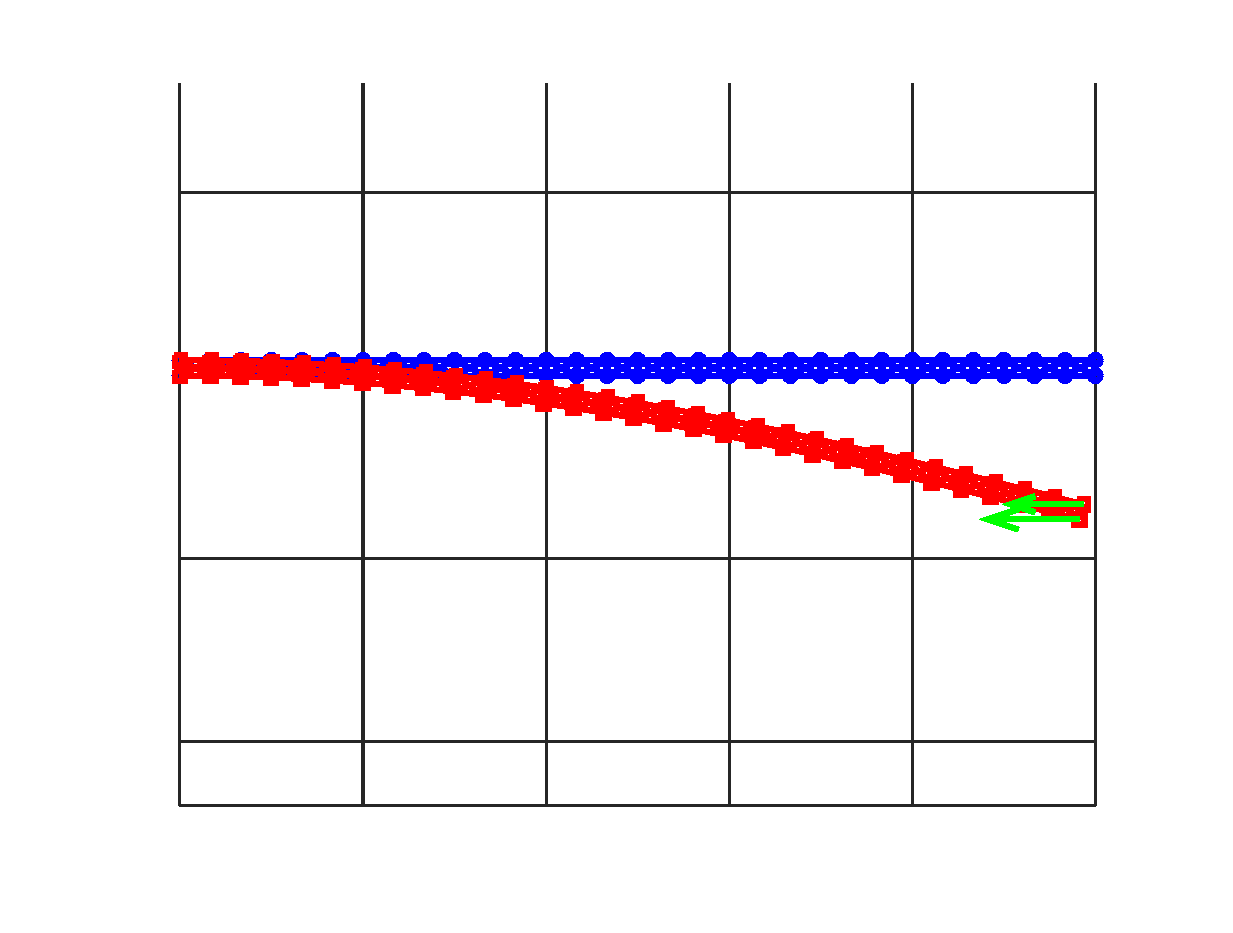
\includegraphics{Cantilever_Buckling_ImperfLoad_deform-inc}
\end{picture}%
\begin{picture}(576,432)(0,0)
\fontsize{20}{0}
\selectfont\put(78.3548,48.007){\makebox(0,0)[t]{\textcolor[rgb]{0.15,0.15,0.15}{{0}}}}
\fontsize{20}{0}
\selectfont\put(166.245,48.007){\makebox(0,0)[t]{\textcolor[rgb]{0.15,0.15,0.15}{{1}}}}
\fontsize{20}{0}
\selectfont\put(254.135,48.007){\makebox(0,0)[t]{\textcolor[rgb]{0.15,0.15,0.15}{{2}}}}
\fontsize{20}{0}
\selectfont\put(342.025,48.007){\makebox(0,0)[t]{\textcolor[rgb]{0.15,0.15,0.15}{{3}}}}
\fontsize{20}{0}
\selectfont\put(429.915,48.007){\makebox(0,0)[t]{\textcolor[rgb]{0.15,0.15,0.15}{{4}}}}
\fontsize{20}{0}
\selectfont\put(517.805,48.007){\makebox(0,0)[t]{\textcolor[rgb]{0.15,0.15,0.15}{{5}}}}
\fontsize{20}{0}
\selectfont\put(73.3497,83.7359){\makebox(0,0)[r]{\textcolor[rgb]{0.15,0.15,0.15}{{-2}}}}
\fontsize{20}{0}
\selectfont\put(73.3497,171.626){\makebox(0,0)[r]{\textcolor[rgb]{0.15,0.15,0.15}{{-1}}}}
\fontsize{20}{0}
\selectfont\put(73.3497,259.516){\makebox(0,0)[r]{\textcolor[rgb]{0.15,0.15,0.15}{{0}}}}
\fontsize{20}{0}
\selectfont\put(73.3497,347.406){\makebox(0,0)[r]{\textcolor[rgb]{0.15,0.15,0.15}{{1}}}}
\fontsize{20}{0}
\selectfont\put(298.08,24.007){\makebox(0,0)[t]{\textcolor[rgb]{0.15,0.15,0.15}{{x}}}}
\fontsize{20}{0}
\selectfont\put(49.3497,226.301){\rotatebox{90}{\makebox(0,0)[b]{\textcolor[rgb]{0.15,0.15,0.15}{{y}}}}}
\end{picture}
}
    	\label{fig:nonlindeform}
    }
	\caption{Resultado numérico obtenido para factor de carga $1$.}
\end{figure}


En la Figura~\ref{fig:nonlindeform} se muestra la estructura en las configuraciones de referencia y deformada (azul y rojo respectivamente).
%
Los gráficos mostrados son los generados por la herramienta ONSA, donde los desplazamientos son graficados en la misma unidad en la que el usuario ingresa las dimensiones, en este caso: metros. %
%
El signo del desplazamiento es considerado opuesto al del sistema de coordenadas del desarrollo analítico, para el gráfico.


Se observa que cuando la carga axial alcanza el valor de carga crítica el desplazamiento del extremo libre alcanza valores relativamente elevados. %
%
Se debe resaltar que el análisis numérico considerado en este ejemplo es no lineal considerando grandes giros, mientras que el resultado analítico considera grandes desplazamientos pero pequeños giros. %
%
Este es el motivo por el cual la flecha tiene a infinito para la carga crítica mientras que numéricamente se observa únicamente un incremento elevado pero finito.

Para finalizar se presenta el resultado numérico obtenido al considerar un factor de carga superior al factor crítico obtenido analíticamente. %
%
En la Figura~\ref{fig:ejpospandeo} se presenta la curva carga-deformación, mientras que en la Figura~\ref{fig:deformpos} se muestra la correspondiente deformada.

\begin{figure}[htb]
	\centering
	\subfloat[Curva carga-desplazamiento.]{
		\resizebox{.5\textwidth}{!}{% Title: gl2ps_renderer figure
% Creator: GL2PS 1.3.9, (C) 1999-2015 C. Geuzaine
% For: Octave
% CreationDate: Sun Dec  3 14:25:11 2017
\setlength{\unitlength}{1pt}
\begin{picture}(0,0)
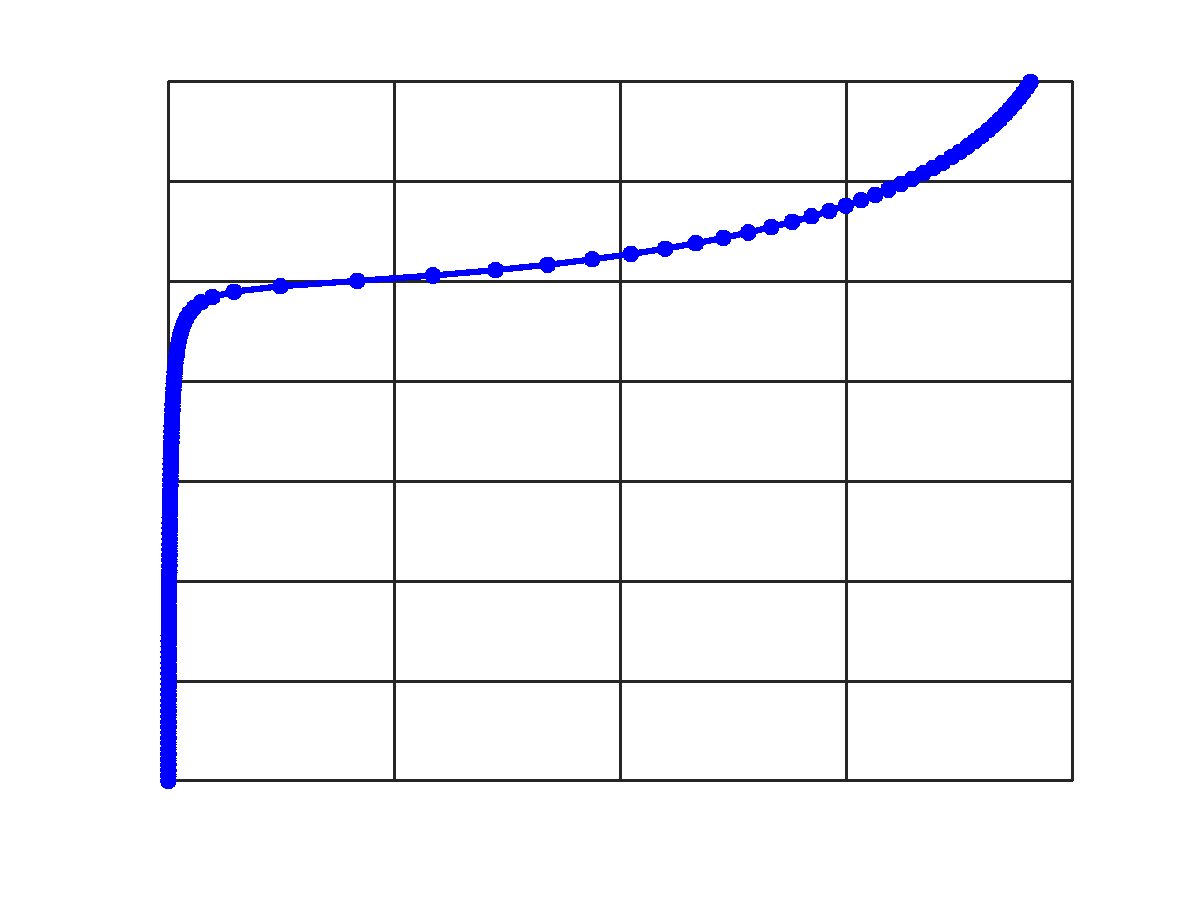
\includegraphics{Cantilever_Buckling_ImperfLoad_pasado-inc}
\end{picture}%
\begin{picture}(560,420)(0,0)
\fontsize{20}{0}
\selectfont\put(72.8,48.007){\makebox(0,0)[t]{\textcolor[rgb]{0.15,0.15,0.15}{{0}}}}
\fontsize{20}{0}
\selectfont\put(181.3,48.007){\makebox(0,0)[t]{\textcolor[rgb]{0.15,0.15,0.15}{{1}}}}
\fontsize{20}{0}
\selectfont\put(289.8,48.007){\makebox(0,0)[t]{\textcolor[rgb]{0.15,0.15,0.15}{{2}}}}
\fontsize{20}{0}
\selectfont\put(398.3,48.007){\makebox(0,0)[t]{\textcolor[rgb]{0.15,0.15,0.15}{{3}}}}
\fontsize{20}{0}
\selectfont\put(506.8,48.007){\makebox(0,0)[t]{\textcolor[rgb]{0.15,0.15,0.15}{{4}}}}
\fontsize{20}{0}
\selectfont\put(67.8,52.9996){\makebox(0,0)[r]{\textcolor[rgb]{0.15,0.15,0.15}{{0}}}}
\fontsize{20}{0}
\selectfont\put(67.8,100.928){\makebox(0,0)[r]{\textcolor[rgb]{0.15,0.15,0.15}{{0.2}}}}
\fontsize{20}{0}
\selectfont\put(67.8,148.857){\makebox(0,0)[r]{\textcolor[rgb]{0.15,0.15,0.15}{{0.4}}}}
\fontsize{20}{0}
\selectfont\put(67.8,196.785){\makebox(0,0)[r]{\textcolor[rgb]{0.15,0.15,0.15}{{0.6}}}}
\fontsize{20}{0}
\selectfont\put(67.8,244.714){\makebox(0,0)[r]{\textcolor[rgb]{0.15,0.15,0.15}{{0.8}}}}
\fontsize{20}{0}
\selectfont\put(67.8,292.643){\makebox(0,0)[r]{\textcolor[rgb]{0.15,0.15,0.15}{{1}}}}
\fontsize{20}{0}
\selectfont\put(67.8,340.571){\makebox(0,0)[r]{\textcolor[rgb]{0.15,0.15,0.15}{{1.2}}}}
\fontsize{20}{0}
\selectfont\put(67.8,388.5){\makebox(0,0)[r]{\textcolor[rgb]{0.15,0.15,0.15}{{1.4}}}}
\fontsize{20}{0}
\selectfont\put(289.8,24.007){\makebox(0,0)[t]{\textcolor[rgb]{0.15,0.15,0.15}{{Displacements}}}}
\fontsize{20}{0}
\selectfont\put(31.8,220.75){\rotatebox{90}{\makebox(0,0)[b]{\textcolor[rgb]{0.15,0.15,0.15}{{Load factors}}}}}
\end{picture}
}
    	\label{fig:ejpospandeo}
	}
	\subfloat[Geometrías de referencia (azul) y deformada (rojo).]{
		\resizebox{.5\textwidth}{!}{% Title: gl2ps_renderer figure
% Creator: GL2PS 1.3.9, (C) 1999-2015 C. Geuzaine
% For: Octave
% CreationDate: Sun Dec  3 14:25:08 2017
\setlength{\unitlength}{1pt}
\begin{picture}(0,0)
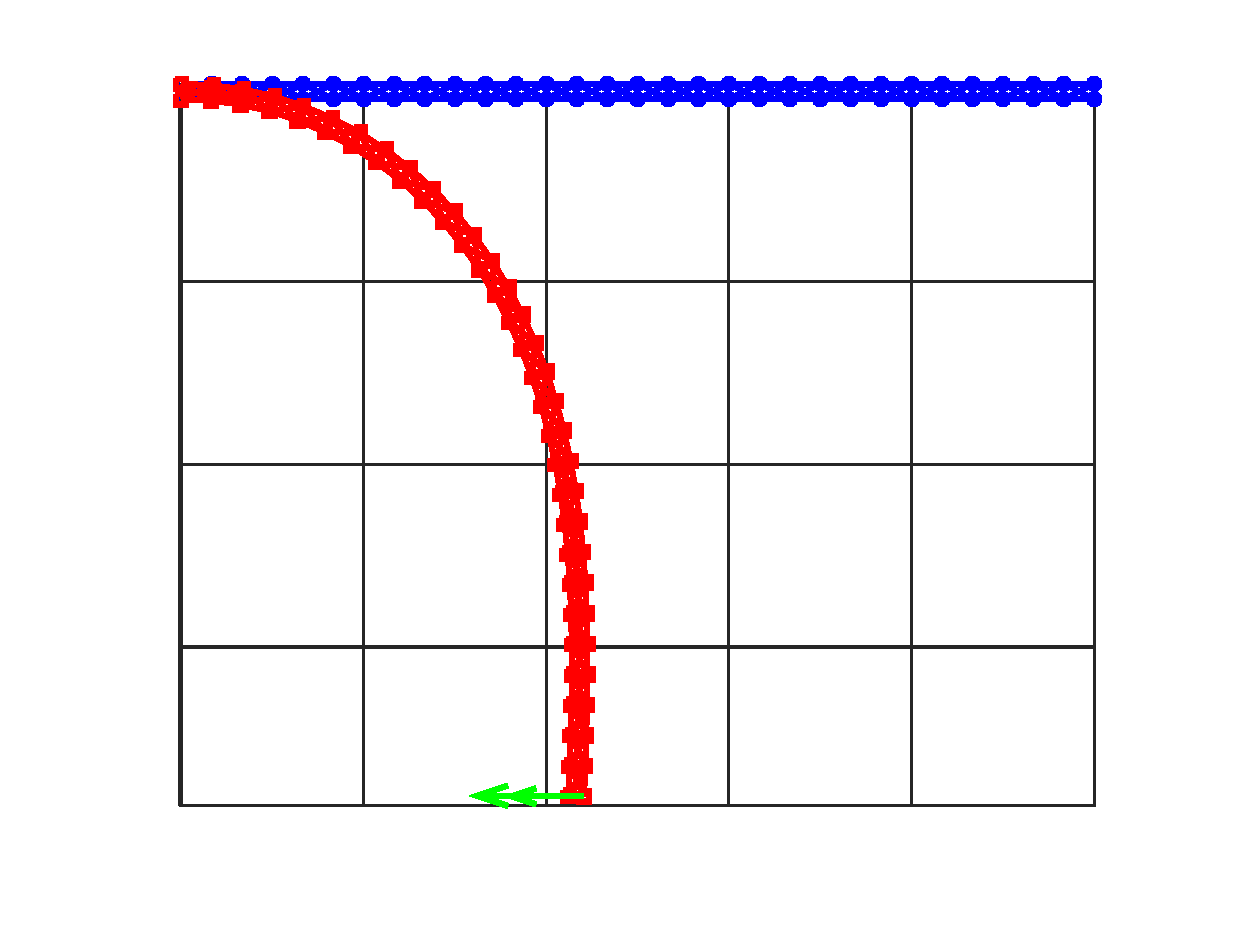
\includegraphics{Cantilever_Buckling_ImperfLoad_pasado_deform-inc}
\end{picture}%
\begin{picture}(576,432)(0,0)
\fontsize{20}{0}
\selectfont\put(78.9711,48.007){\makebox(0,0)[t]{\textcolor[rgb]{0.15,0.15,0.15}{{0}}}}
\fontsize{20}{0}
\selectfont\put(166.615,48.007){\makebox(0,0)[t]{\textcolor[rgb]{0.15,0.15,0.15}{{1}}}}
\fontsize{20}{0}
\selectfont\put(254.258,48.007){\makebox(0,0)[t]{\textcolor[rgb]{0.15,0.15,0.15}{{2}}}}
\fontsize{20}{0}
\selectfont\put(341.902,48.007){\makebox(0,0)[t]{\textcolor[rgb]{0.15,0.15,0.15}{{3}}}}
\fontsize{20}{0}
\selectfont\put(429.545,48.007){\makebox(0,0)[t]{\textcolor[rgb]{0.15,0.15,0.15}{{4}}}}
\fontsize{20}{0}
\selectfont\put(517.189,48.007){\makebox(0,0)[t]{\textcolor[rgb]{0.15,0.15,0.15}{{5}}}}
\fontsize{20}{0}
\selectfont\put(73.3497,129.277){\makebox(0,0)[r]{\textcolor[rgb]{0.15,0.15,0.15}{{-3}}}}
\fontsize{20}{0}
\selectfont\put(73.3497,216.92){\makebox(0,0)[r]{\textcolor[rgb]{0.15,0.15,0.15}{{-2}}}}
\fontsize{20}{0}
\selectfont\put(73.3497,304.564){\makebox(0,0)[r]{\textcolor[rgb]{0.15,0.15,0.15}{{-1}}}}
\fontsize{20}{0}
\selectfont\put(73.3497,392.208){\makebox(0,0)[r]{\textcolor[rgb]{0.15,0.15,0.15}{{0}}}}
\fontsize{20}{0}
\selectfont\put(298.08,24.007){\makebox(0,0)[t]{\textcolor[rgb]{0.15,0.15,0.15}{{x}}}}
\fontsize{20}{0}
\selectfont\put(49.3497,226.301){\rotatebox{90}{\makebox(0,0)[b]{\textcolor[rgb]{0.15,0.15,0.15}{{y}}}}}
\end{picture}
}
		\label{fig:deformpos}
	}
	\caption{Resultado numérico de comportamiento post-pandeo, factor de carga máximo: $1.4$.}
\end{figure}

Se puede observar el comportamiento de rigidización post-pandeo de la estructura, el cual no puede ser reproducido por el modelo de pequeños giros considerado para el cálculo analítico. %
%
Se destaca que el comportamiento post-pandeo observado corresponde a un material con un comportamiento constitutivo elástico lineal. Materiales como acero y hormigón tienen un comportamiento no lineal por lo que la elástica para grandes giros puede ser diferente, por ejemplo a través de la formación de una rótula plástica en el empotramiento.